\documentclass{article}
\usepackage{listings}
\usepackage{algorithm}
\usepackage{algorithmic}
\usepackage{graphicx}
\usepackage{circuitikz}
\usepackage{tikz}
\usepackage{pgfplots}
\usepackage{subcaption}
\usepackage{setspace}
\usepackage{indentfirst}
\usepackage{siunitx}
\usepackage{titlesec}
\usepackage{amsmath}
\usepackage[title]{appendix}
\usepackage[backend=bibtex,style=ieee]{biblatex}
\usepackage[english]{babel}
\usepackage[autostyle, english = american]{csquotes}
\MakeOuterQuote{"}
\usepackage{pbox}
\newcommand{\ctikzlabel}[2]{\pbox{\textwidth}{#1\\#2}} % multiple-lines labels
\usepackage{relsize}
\tikzset{
    pin/.style = {font = \relsize{-2}} % pin font size
}
\ctikzset{
    bipoles/length = 2em, % bipole size
    font = \relsize{-1}, % default font size
}
\floatname{algorithm}{Algorithm}
\renewcommand{\algorithmicrequire}{\textbf{Input:}}
\renewcommand{\algorithmicensure}{\textbf{Output:}}
\usepackage[margin=1in]{geometry}
\usetikzlibrary{calc}
\usetikzlibrary{intersections}
\addbibresource{Interim_Report_References.bib}
\DeclareSIUnit{\ft}{'}
\DeclareSIUnit{\in}{"}
\usepackage{lipsum}
\doublespacing
\renewcommand{\thesection}{\arabic{section}}
\renewcommand{\thesubsection}{\arabic{subsection}}
\renewcommand{\thesubsubsection}{\arabic{subsubsection}}
\pgfplotsset{compat=1.13}
% \titleformat{\section}[block]{\centering}{}{}
\titlelabel{\thetitle.\quad}
\titleformat{\section}[block]{\large\filcenter}{\thesection.}{1em}{}
\titleformat{\subsection}{\large\filright}{\thesection.\thesubsection.}{1em}{}
\titleformat{\subsubsection}{\normalsize\filright}{\thesection.\thesubsection.\thesubsubsection.}{1em}{\itshape}
% \titleformat{\subsection}{\normalfont\large}{\thesubsection.}{1em}{}

\title{
     {Autonomous Robotic Team Sports Swarm}
}
\author{Nicholas Gregg, Noah Pratt, Victoria Rodriguez, Rick Trevino \\ Texas Tech University}
\date{October 2018}
\begin{document}
% Title Page
     \thispagestyle{empty}
     \maketitle
     \newpage
% Abstract
     % \begin{abstract}
     \section*{Abstract}
          % \lipsum[1-2]
          % FIX THIS!!!!!!!!!
          This report details the methods used to enable three autonomous robots to compete in a soccer-like game against an opposing team of three robots while communicating and receiving information over a wireless network. Each rover design uses the Raspberry Pi Zero W to wirelessly connect to an Ubuntu Linux computer acting as the central hub and communicates information using standard libraries in the Robot Operating System (ROS). The central hub periodically queries a wireless MyRIO server for JSON files that contain coordinate data for the field’s corners, the ball, and all soccer players. This coordinate data is provided to the wireless server via an overhead camera in a vision system that was provided for use by Derek A. Johnston. Once the central computing hub receives this coordinate data, ROS is used to analyze the data, make calculations, and broadcast decisions to the Raspberry Pis on the rover units. Using these methods, each player is capable of chasing the ball,  kicking the ball, receiving a pass, avoiding other players, blocking enemy shots, or completing various other tasks.
          % This paper details the methodology of designing a robotic swarm of three autonomous units capable of a participating in a soccer match on a \SI{4x8}{\ft} field and using a \SI{3}{\in} diameter plastic “ball pit” ball. Each robot unit is designed to fit within a cylindrical volume constraint of \SI{8}{\in} tall cylinder with a diameter of \SI{8}{\in} and to hold a \SI{1/4}{\in} thick, \SI{8}{\in} diameter disk that is seen by an overhead camera that provides player coordinate data via a provided vision system. The three units are wirelessly connected over Wi-Fi to a central computing hub which relays motor commands to the units based on information the hub receives from said vision system.
     % \end{abstract}
     \newpage
% Table of Contents
     \tableofcontents
     \newpage
% List of Figures
     \listoffigures
     % \newpage
     % \vspace*{\stretch{1}}
     \listofalgorithms
     \newpage
% List of Tables
     \listoftables
     \newpage
% Introduction
     \section{Introduction}
     % \lipsum[1-2]
     % The individual units of the swarm act as single agents and are each only capable of performing simple tasks, controlled by a clear set of rules and local stimuli \cite{Zheng13}.

     % Introduction:
     % Background on what swarm robotics is
     The strategy of implementing swarm-like behavior into several small, simple machines is called \textit{swarm robotics}. This approach is characterized by its robustness, flexibility, and scalability \cite{Sahin08}. These characteristics enable the group of robots, referred to as the swarm, to achieve complex, collective tasks despite a distinct lack of highly developed intelligence in the individual units of the swarm \cite{Zheng13}.
     % Objective of paper
     \par This paper discusses the methodology behind a design and implementation of this strategy with the objective of demonstrating capability in playing soccer. In this design, the swarm is comprised of three homogeneous units, each of which is only responsible for navigation. The more complex algorithms are performed by a central hub which broadcasts information to the individual agents. The central hub (a laptop running Xenial Ubuntu 16.04) receives the location of each of the units of the swarm from an overhead camera and vision system; this system broadcasts pixel coordinates in a JavaScript Object Notation (JSON) file from the camera image of all expected obstacles on the field (two swarms of 3 units, each unit marked by a colored shape against the field of a white \SI{4x8}{\ft} table).
     % Description of the central hub <--> vision system
     The laptop then executes several Python scripts which store these pixel coordinates, translate them to coordinates on the field, and mark their translated coordinates on a map which is broadcast to the units of the swarm; the units then use this map to avoid collisions between one another. This map is called a \textit{costmap}: an occupancy grid which updates itself when coordinates of obstacles change and marks obstacles on the map accordingly for path planning algorithms to use when deciding on a path to take \cite{costmap_2d}. This map is maintained throughout the runtime of the system as a vital component of the \textit{navigation stack}, a popular set-up using several key packages in the Robot Operating System (ROS) framework that is used to provide a clear path solution at any moment in time.
     \par The overhead camera and vision system is significantly limited in several distinct ways \cite{ProjectDescription}:
     \begin{enumerate}
          \item It has an exceptionally slow update rate of approximately \SI{1}{\hertz}.
          \item It cannot host more than 3-4 connections with any stability.
          \item The algorithm it uses for tracking objects relies on the contrast between brightly colored shapes against a plain white background. This requires the boundary of a white border around the colored shape at all times.
     \end{enumerate}
     % Addressing each constraint
     % First constraint: slow update rate
     \par The design described in this paper attempts to address each of these constraints. The first constraint is addressed by using encoders on each of the units to track their locations on the field, using the coordinates from the vision system to account for the drift that would occur over time from the position determined by the vision system to the position determined by the encoders \cite{REP105}.
     % Second constraint: can't host more than 3
     \par The second constraint is addressed by utilizing a \textit{centralized} system design, wherein the units of the swarm do not communicate with each other but instead communicate only to a central hub connected to each unit of the swarm.
     % Background on how swarm robotics is usually implemented and why we chose differently
     Historically, swarm robotics is typically implemented as a \textit{distributed} system \cite{Dimos08}\cite{Easton04}, and Sahin argues that it is one of the defining characteristics of swarm robotics \cite{Sahin08}. However, in addition to addressing the second constraint of the vision system, the centralized system design provides two main advantages: it is achieved in a simple structure, and it guarantees an optimized solution, as the central hub is connected to all units of the swarm at once and can thus take all parameters into account \cite{Barca16}. For these reasons, it was decided that the centralized design was more practical for the application of playing soccer than a distributed system design.
     % Third constraint: volume
     \par To address the third constraint of the vision system, each unit is confined to a cylindrical volume of \SI{8}{\in} height with diameter of \SI{8}{\in} and holds an \SI{8}{\in} diameter, \SI{1/4}{\in} thick disk such that each unit is completely covered under the disk. This disk is completely white with the brightly colored shape in the center, ensuring that the vision system would not see an overlap of shapes when two units collide; the disk provides a white border around the colored shape at all times.
     \par This paper will discuss the setup of the network on which the central hub communicates with the swarm, the algorithms of the Python scripts executed by the central hub, and the navigation stack responsible for path-planning around the field. Testing of the methods described in this paper will use a simplified version of soccer: there will only be two rounds and each one has a duration of three minutes. No penalties are considered in tracking ``points'' scored by a team.

% Methodology
     \section{Methodology}
     % \lipsum[1]
     % Basic ROS concepts
     The design in this system utilizes the simplicity and effectiveness of the ROS framework for communication between the central hub and each unit of the swarm. The ROS framework uses \textit{nodes} (executables within a ROS package) to subscribe to and publish \textit{messages} (simple data structure comprised of typed fields) over \textit{topics} (uniquely named buses used to exchange information). This structure of communication is used extensively in the methods described in this paper.
     % Basic description of what an ad-hoc is
     % \par The network connections are set up using a heterogeneous wireless Ad-Hoc network (WANET), which does not rely on infrastructure such as routers or access points. Instead, members of the network participate in direct peer-to-peer (p2p) communication and file sharing, and each network is configured dynamically, allowing for anytime and anywhere computing \cite{Mishra08}. The central computing hub is wirelessly connected to the TTUSwarmField myRIO network, which is already configured in infrastructure mode, independently of the Ad-Hoc network, so that the Ad-Hoc network consists only of the central hub and player nodes. This can be accomplished by either using a network adapter that supports host mode, or by using two seperate network adapters entirely. The central hub runs an Ubuntu Linux 16.04 virtual machine in order to run ROS and broadcasts a wireless Ad-Hoc network using the onboard network adapter. Each player is able to connect to this network using the Raspberry Pi Zero W, and the virtual machine is able to connect via IP forwarding from the Windows host.

     \par To properly utilize the ROS framework, a laptop (separate from the one used as the central hub) that is connected to the network hosted by the vision system is used as a wireless access point (WAP); this allows the central hub to connect to the projected network and perform all of the necessary operations on a separate network than the one used by the vision system to broadcast the JSON file. This separation from the network is desirable as the network hosted by the vision system is unstable and can only host three connections at a time \cite{ProjectDescription}.

     % Basic description of JSON Grabber
     \par From this separate network, the central hub sends "get" requests to the address on the vision system network which broadcasts the JSON file, publishes the data from the JSON file onto unique ROS topics, converts these coordinates from the set of pixels to the set of coordinates on the table, and uses these converted coordinates to track the units of the swarm.
     % Basic description of parameter server and launch files?
     % These Python scripts are launched in XML "launch" files: a type of file using XML syntax that can be used to launch multiple nodes at once. These launch files also launch parameter servers. The parameter servers are used with the modular design of each of the scripts; each script is designed for the most generic case such that the parameter servers can be later configured for the script for a more specific case (e.g. publishing JSON data to a different topic for each different unit of the swarm).
     % Materials on each rover
     \begin{figure}[h]
          \centering
          \begin{subfigure}{0.4\textwidth}
               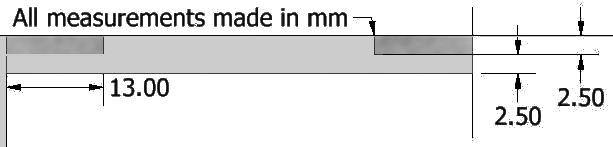
\includegraphics[scale=0.25]{images/hat_1}
          \end{subfigure}
          \begin{subfigure}{0.4\textwidth}
               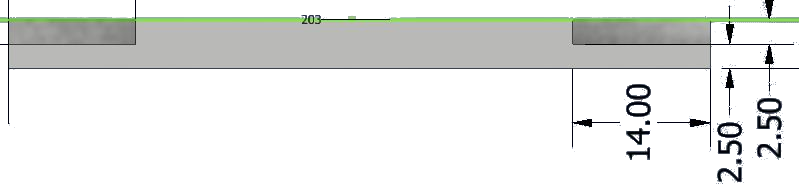
\includegraphics[scale=0.2]{images/hat_2}
          \end{subfigure}
          \begin{subfigure}{0.4\textwidth}
               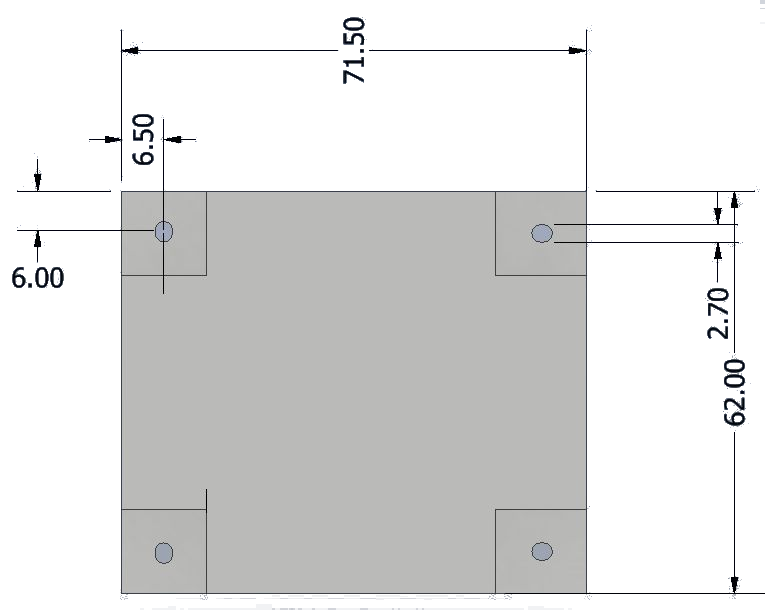
\includegraphics[scale=0.25]{images/hat_3}
          \end{subfigure}
          \caption[Blueprint of 3D Printed Stand]{Image created in AutoCAD Inventor.}
          \label{fig:hat-holder}
     \end{figure}
     \par Equipped on each unit of the swarm is a portable single-board computer connected to a control board which has both a motor driver circuit and a power distribution system on board. The computer is used to run two Python scripts: the first subscribes to topics with messages published by the central hub containing velocity commands which the computer translates into motor commands, the second is to publish data from the encoders and gyroscope onto a topic for the central hub to subscribe to so that it can perform the more advanced calculations. Additionally, each unit is equipped with a solenoid "kicker" used to kick the ball toward the goal and a 3D printed stand (see Figure \ref{fig:hat-holder}) designed to sit atop the unit and hold the \SI{8}{\in} disk described earlier. This stand uses a micro-suction adhesive: a non-stick solution to holding the disk securely without risk of damaging the disk that uses small bubbles of air throughout the surface of the tape; these bubbles are squeezed out when an object is pressed onto them, creating a vacuum seal to the object \cite{Crawford17}.
          % \subsection{Network Set-Up}
          % \lipsum[1]
          % \newpage
          \subsection{Solenoid Kicker}
          % \lipsum[1]
          Each unit is equipped with a plow and solenoid. The plow prevents the ball from drifting away from the units while moving or turning. The solenoid allows the units to move the ball large distances across the field by applying physical force to the ball.
          \par The solenoid is controlled using the circuit seen in Figure  \ref{fig:sol-ckt}. The circuit uses a boost converter, tuned to output \SI{45}{\volt} with the trim resistor to charge a capacitor. When the solenoid needs to be activated by the unit, a single pulse signal is sent to the relay at $S_1$, which closes the connection between the solenoid and the capacitor. This discharges the capacitor into the solenoid, causing the piston to extend momentarily. Once this occurs, and the signal pulse ends, the connection between the capacitor and the boost converter closes, and the connection between the solenoid and the capacitor opens. The boost converter is then able to recharge the capacitor so the process can be repeated.
          \begin{figure}[H]
               \centering
               \begin{circuitikz}[american voltages]
                    \draw [thick] (4,0) coordinate (u1) rectangle ++(2,3); % shape
                    \draw [pin] (u1) ++ (1,3) coordinate (u1 vcc)
                         node[below]{$V_{CC}$}
                         node[above left]{3}; % VCC
                    \draw [pin] (u1) ++ (1,0) coordinate (u1 gnd)
                         node[above]{GND}
                         node[below left]{1}; % GND
                    \draw [pin] (u1) ++ (0,2) coordinate (u1 sgnd)
                         node[right]{SGND}
                         node[above left]{5}; % SGND
                    \draw [pin] (u1) ++ (0,1) coordinate (u1 trim)
                         node[right]{TRIM}
                         node[above left]{6}; % TRIM
                    \draw [pin] (u1) ++ (2,1.5) coordinate (u1 vout)
                         node[left]{$V_{\text{out}}$}
                         node[above right]{2}; % VOUT
                    \draw (u1) ++ (2,0)
                         node[right]{\ctikzlabel{$U_1$}{ABXS001}};
                    \draw (u1 vcc) -- ++(0,1) -- ++(-4,0) coordinate (top bat);
                    \draw (u1 gnd) -- ++(0,-1) -- ++(-4,0) coordinate (bot bat);
                    \draw (u1 sgnd) -- ++(-1.5,0) coordinate (top rtrim);
                    \draw (u1 trim) -- ++(-1.5,0) coordinate (bot rtrim);
                    \draw (top rtrim) to [R,l=$\SI{5.6}{\kilo\ohm}$] (bot rtrim);
                    \draw (top bat) to [battery, l=9 V] (bot bat);
                    \draw (u1 gnd) -- ++(0,-1) -- ++(4,0) coordinate (bot cap);
                    \draw (bot cap) -- ++(2,0) coordinate (bot sol);
                    \draw (bot cap) to [pC, l_=$\SI{680}{\micro\farad}$] ++(0,1.5) coordinate (start sw);
                    \draw[draw=none] (start sw) -- ++(0,0.5) coordinate (start sw1);
                    \draw (start sw1) node[spdt,rotate=90](Sw){};
                    \draw (Sw.in) -- (start sw);
                    \draw (Sw.out 1) -- ++(0,0.2) -- ++(-1,0) coordinate (sw out 1);
                    \draw (Sw.out 2) -- ++(0,0.2) -- ++(1,0) coordinate (sw out 2);
                    % \draw (sw out 1) |- (u1 vout);
                    \draw (u1 vout) to [R,l=$\SI{45}{\ohm}$]++(2,0) coordinate (rlimit out);
                    \draw (rlimit out) to (sw out 1);
                    \draw (bot sol) to [L,l_=Solenoid] ++(0,2.25) coordinate (top sol);
                    \draw (top sol) |- (sw out 2);
                    \draw (u1 gnd) to [short,-*] ++(0,-1) node[ground]{};
                    \draw[draw=none] (Sw.in) -- ++(0.25,0) coordinate (label sw);
                    \draw (label sw) to [open,l=$S_1$]++(0.25,0);
               \end{circuitikz}
               \caption[Solenoid Charge Circuit Schematic]{Schematic of the solenoid charge circuit. Uses an ABXS001 boost converter.}
               \label{fig:sol-ckt}
          \end{figure}
          \subsection{Power Distribution}
          \begin{table}[h]
          \begin{tabular}{lllll}
            Name                           & Quantity & Operating Voltage (Typ.) & Current Draw & Power Consumption \\
            Pololu 120:1 Gearmotor         & 2        & 4.50 V                   & 0.80 A       & 7.20 W            \\
            Pololu Romi 32U4 Control Board & 1        & 7.20 V                   & 0.20 A       & 1.44 W            \\
            Raspberry Pi Zero W            & 1        & 5.00 V                   & 1.00 A       & 5.00 W            \\
            Solenoid Charge Circuit        & 1        & 12.00 V                  & 1.00 A       & 12.00 W           \\
            \textit{Unused Power}          & \multicolumn{3}{l}{}                               & 11.47 W
          \end{tabular}
          \label{tab:power-dist}
          \end{table}
          The solenoid is
          \subsection{Coordinate Conversion}
          % \lipsum[1]
          To map the set of pixel coordinates given by the JSON file (referred to from this point onward as set $S_p$) to the set of physical coordinates on the table (referred to from this point onward as set $S_t$), a bijective 2D \textit{homography} is constructed. Gava and Bleser define a 2D homography as "an invertible mapping $h$ from $P^2$ to itself such that three points $x_1$, $x_2$, $x_3$ lie on the same line if and only if $h_1(x)$, $h_2(x)$, $h_3(x)$ do," and they theorize that "a mapping $h$ from $P^2\rightarrow P^2$ is a homography if and only if there exists a non-singular \num{3x3} matrix $H$ such that for any point in $P^2$ represeted by a vector $x$ it is true that $h(x)=Hx$ \cite{GavaDfki}." In other words, if each $x_i'$ is an element in the set $S_p$ and each $x_i$ is an element in the set $S_t$, then
          \begin{equation}
               \begin{pmatrix}
                    x'_1\\
                    x'_2\\
                    x'_3
               \end{pmatrix}
               =
               \begin{bmatrix}
                    h_{1,1} & h_{1,2} & h_{1,3} \\
                    h_{2,1} & h_{2,2} & h_{2,3} \\
                    h_{3,1} & h_{3,2} & h_{3,3}
               \end{bmatrix}
               \begin{pmatrix}
                    x_1 \\
                    x_2 \\
                    x_3
               \end{pmatrix}
          \end{equation}
          which is also equivalent to $S_p(x')=H\,S_t(x)$ and takes the form of the standard linear equation $Ax=b$. For the 2D case, the last element in the vector of physical coordinates on the table $x'_3$ is assumed to be 1. As a result, the last element in the homography matrix $h_{3,3}$ is also 1. Thus, the homography matrix has 8 degrees of freedom (DOF).
          \begin{equation}
               \begin{bmatrix}
                    x_i'\\
                    y_i'\\
                    1
               \end{bmatrix}
               =
               \begin{bmatrix}
                    h_{1,1} & h_{1,2} & h_{1,3} \\
                    h_{2,1} & h_{2,2} & h_{2,3} \\
                    h_{3,1} & h_{3,2} & 1
               \end{bmatrix}
               \begin{bmatrix}
                    x_i\\
                    y_i\\
                    1
               \end{bmatrix}
          \label{eqn:homography1}
          \end{equation}
          \par With 8 DOF, at least four known matches between $S_p$ and $S_t$ are required for a minimal solution for $H$ \cite{GavaDfki,HomographyLab}. For the purposes of this paper, these four points in the set $S_p$ and its known $S_t$ mapping relate to the corners of the table. The pixel coordinates of each corner are received from the JSON file and are manually related to a corresponding coordinate in $S_t$ where the coordinates of the corners are in meters of the physical dimensions of the actual table. This process of manually mapping the corners to solve for the homography matrix is called \textit{four-point parameterization} \cite{Baker11}, and for the methods described in this paper, it occurs each time the pixel coordinates of the table change so that the homography matrix can be re-calibrated. It can be shown that the previous equation can be expressed as
          \begin{equation}
               \begin{bmatrix}
                    x_i & y_i & 1 & 0 & 0 & 0 & -x_i'\cdot x_i & -x_i'\cdot y_i \\
                    0 & 0 & 0 & x_i & y_i & 1 & -y_i'\cdot x_i & -y_i'\cdot y_i
               \end{bmatrix}
               \cdot
               \begin{bmatrix}
                    h_{1,1} \\ h_{1,2} \\ h_{1,3} \\
                    h_{2,1} \\ h_{2,2} \\ h_{2,3} \\
                    h_{3,1} \\ h_{3,2}
               \end{bmatrix}
               =
               \begin{bmatrix}
                    x_i'\\
                    y_i'\\
               \end{bmatrix}
          \label{eqn:homogeneous_eqn}
          \end{equation}
          for each corner $i$; the dimension of the \num{2x8} matrix becomes \num{8x8} during the four-point parameterization, and allows the linear equation to be solved for the column vector $h$. Once $h$ is found, its elements can be used with the linearly independent equations derived from Equation \ref{eqn:homogeneous_eqn}:
          \begin{align}
               x_i'&=\frac{h_{1,1}x_i+h_{1,2}y_i+h_{1,3}}{h_{3,1}x_i+h_{3,2}y_i+1}\\
               y_i'&=\frac{h_{2,1}x_i+h_{2,2}y_i+h_{2,3}}{h_{3,1}x_i+h_{3,2}y_i+1}
          \end{align}
          to solve any new pixel coordinate given a physical coordinate on the table\cite{GavaDfki,HomographyLab}. After converting the column vector $h$ back into the square matrix $H$ (substituting the last element $h_{3,3}$ for 1), the inverse matrix $Q$ can be calculated; the inverse matrix $Q$ can be used to calculate the matching physical coordinates on the table given any pixel coordinate:
          \begin{align}
               x &= \frac{q_{1,1}x'+q_{1,2}y'+q_{1,3}}{q_{3,1}x'+q_{3,2}y'+q_{3,3}}\\
               y &= \frac{q_{2,1}x'+q_{2,2}y'+q_{2,3}}{q_{3,1}x'+q_{3,2}y'+q_{3,3}}
          \label{eqn:inverse_eqn}
          \end{align}
          The four-point parameterization and re-calculation of the homography matrix occurs at every update of the pixel coordinates of the four corners on the table, as described in Algorithm \ref{alg:hom_calib}. All other Python scripts which require converting a pixel coordinate to its matching coordinate in the set $S_t$ uses Equations 6 and \ref{eqn:inverse_eqn} to calculate the physical coordinate.
          \begin{algorithm}[H]
               \caption[Homography Calibrater]{Four-point parameterization of the homography matrix.}
               \label{alg:hom_calib}
               \begin{algorithmic}[1]
                    \REQUIRE Pixel coordinates of each corner of the table from the JSON file.
                    \ENSURE Homography matrix and inverse homography matrix.
                    \FOR{each update of the input}
                    \STATE Store each pixel corner coordinate.
                    \STATE Set the table corner coordinates to the corners of a \SI{4x8}{\ft} rectangle (converted to meters).
                    \STATE Construct a column vector $b$ of the pixel coordinates taken from the JSON file.
                    \STATE Construct a \num{8x8} matrix $A$ from the coordinates of the corners in both sets of points (pixels \textit{and} table).
                    \STATE Solve the equation $Ax=b$ for the \num{8x1} column vector $x$.
                    \STATE Make a square matrix from the resulting column vector $x$, with the last element in the \num{3x3} matrix just being 1.
                    \STATE Store this square matrix as the homography matrix.
                    \STATE Find the inverse of the new square matrix.
                    \STATE Store this square matrix as the inverse homography matrix.
                    \STATE Publish both matrices.
                    \ENDFOR
               \end{algorithmic}
          \end{algorithm}
          \subsection{Navigation Stack}
          % The navigation stack assumes a specific configuration and is used in common ROS navigation packages such as move_base and amcl. The overview of this configuration is illustrated in Figure #. The required nodes (sensor sources, sensor transforms, odometry source, and base controller) are each used by the nodes provided in the navigation package. The navigation package uses the sensor sources (streams of data from a sensor, typically Lidar, in the form of a LaserScan or a PointCloud) to populate a costmap that is generated by the package. This costmap is used to map the environment around the rover by the likelihood that an obstacle exists in each cell of the map; these probabilities are calculated from the sensor streams. The costmap is broken into global and local components, with the local component used for immediate path planning and the global component used for long-term path planning. For example, the global planner might instruct the rover to move from point A to point B, but the local planner instructs the rover to first avoid the obstacle immediately in front of it. The odometry source is used for the local planner while the sensor sources are used for both the global and local path planner. The base controller subscribes to the velocity commands given by the path planners and converts them to motor commands on the control board.
          The navigation stack is a framework that uses information provided from odometry sources and sensors of the environment around the robot to plan paths for the robot in the environment that is free of obstacles \cite{ROSNav}. It assumes a specific configuration for the information it is receiving:
          \begin{itemize}
          \item The robot is publishing information from odometry sources (e.g. encoders) to the \verb|odom| topic.
          \item The robot has a planar sensor mounted on top of it that is publishing information in a sensor stream, either in the format of PointCloud or LaserScan.
          \item The robot can take in velocity commands and output the appropriate velocity in the motors using a node called \verb|base_controller|.
          \item The transform from the sensor to its position on the rover is defined and published in the \verb|/tf| transform tree.
          \end{itemize}
          These requirements are addressed as various nodes that publish to expected topics for the nodes in the navigation stack to subscribe to (see Figure \ref{fig:nav-stack-overview}). An odometry node subscribes to the topics that a separate node running from the computer on each unit is publishing information to such as the center displacement of the unit and its linear and angular velocities. The odometry node then fills an \verb|nav_msgs/Odometry| message with the appropriate information so that it can publish to the \verb|odom| topic that the navigation stack is subscribed to.
          \par There are no planar sensors mounted on each unit, so to address this requirement, sensor streams are generated using the coordinates of obstacles surrounding each unit from the JSON file. These sensor streams are then used to construct the costmap of the obstacles around each unit. Since there are no physical sensors on the rover, the requirement of creating a transform for each sensor is fulfilled by using a \textit{static broadcaster} which broadcasts a transform that is rigidly attached at a fixed coordinate (the origin of the coordinate frame of the rover).
          \par The \verb|base_controller| node subscribes to the velocity commands published by the \verb|move_base| node in the navigation stack and translates velocity to motor commands. The \verb|move_base| node that publishes these velocity commands uses the costmap that was constructed using the sensor streams to plan a path that is free of obstacles, and steers the unit onto that path by providing velocity commands along that path.
          \begin{figure}[h]
               \centering
               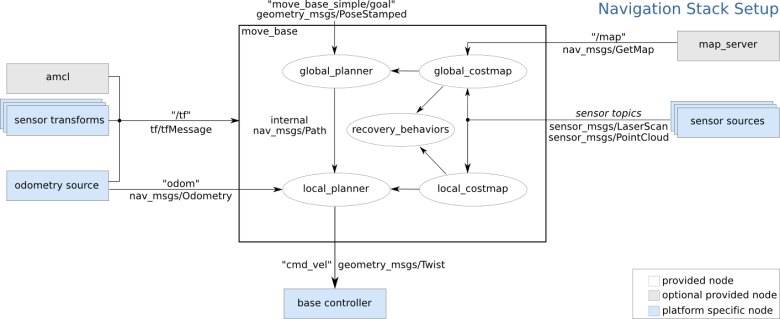
\includegraphics[scale=0.5]{images/nav_stack_overview}
               \caption[Overview of the Navigation Stack Setup]{Overview of the nodes used by the navigation stack.}
               \label{fig:nav-stack-overview}
          \end{figure}
          \subsubsection{Base Controller}
          The unit is controlled using linear and angular velocity commands published by the \verb|move_base| node provided by the navigation stack. These velocity commands are converted from m/s to ft/s. The minimum and maximum velocity of the rover was measured to be -0.78508 and 0.78508 ft/s respectively. These values are used to map the range of velocities in ft/s to the minimum and maximum motor command provided by the motor control libraries from the control board \cite{pololu} using Equation \ref{eqn:range_setter}.
          \begin{equation}
            y = (x-a)\frac{d-c}{b-a}+c
          \label{eqn:range_setter}
          \end{equation}
          \par The linear velocity is used as a baseline for both motors. The angular velocity added to the right motor and subtracted from the left motor, decreasing or increasing the value depending on the sign. Positive angular velocity indicates a counterclockwise motion and negative angular velocity indicates a clockwise motion.

          \subsubsection{Odometry Source}
          % \lipsum[1]
          The navigation stack subscribes to an odometry message on the \verb|odom| topic. The odometry message contains the position and the linear and angular velocity that are calculated using the odometry sources. For the methods described in this paper, the odometry sources are the encoders of the motors and a gyroscope. The encoders are utilized to calculate the displacement in each wheel by using a conversion rate of 1,440 encoder counts for each complete revolution of the motor \cite{PololuEncoders}.
          \begin{figure}[H]
               \centering
               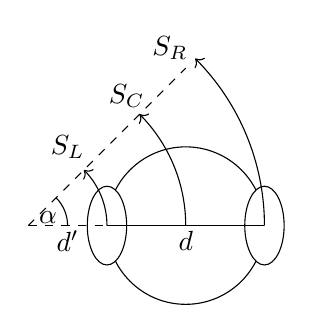
\begin{tikzpicture}
                    \draw (0,0) circle [radius=1cm];
                    \draw[fill=white] (-1,0) circle [x radius=0.25cm, y radius=0.5cm];
                    \draw[fill=white] (1,0) circle [x radius=0.25cm, y radius=0.5cm];
                    \draw[->] (-1cm,0) arc [start angle=0, end angle=45, radius=1cm];
                    \draw (-1.5cm,1) node {$S_L$};
                    \draw[->] (0,0) arc [start angle=0, end angle=45, radius=2cm];
                    \draw (-.75cm,1.65) node {$S_C$};
                    \draw[->] (1cm,0) arc [start angle=0, end angle=45, radius=3cm];
                    \draw (-.2,2.25) node {$S_R$};
                    \draw (-1.5cm,0) arc [start angle=0, end angle=45, radius=0.5cm];
                    \draw (-1.75cm,0.1) node {$\alpha$};
                    \draw (-1,0) -- (1,0);
                    \draw (0,-0.2) node {$d$};
                    \draw (-1.5cm,-0.2) node {$d'$};
                    \draw[dashed] (-2,0) -- (0,2);
                    \draw[dashed] (-2,0) -- (1,0);
               \end{tikzpicture}
               \caption[Odometry Calculation Demonstration]{Demonstration for the calculation of the orientation \cite{DiffSteering}.}
               \label{fig:odom-demo}
          \end{figure}
          In the general case, the angular displacement of the rover's facing direction $\alpha$ is calculated with the encoders as
          \begin{equation}
               \alpha = \frac{S_R-S_L}{d}
          \end{equation}
          where $S_R$ is the displacement of the faster wheel, which is also the wheel furthest from the pivot, and $S_L$ is the displacement of the slower wheel. In the specific case that one of the wheels is stationary, $S_L=0$ and the equation reduces to $S_R/d$. Otherwise, if both wheels move at the same speed, creating a linear path of motion, then $S_R=S_L$ and $\alpha=0$. The angular displacement $\alpha$ is also calculated using the gyroscope on the inertial measurement unit (IMU) of the control board. The gyroscope outputs in \si{\milli\degree\per\s} \cite{LSM6DS33}, which is converted to degrees through the equation $\sum_{t=0}\Delta\theta T_s$ where $T_s$ is the sampling period (\SI{0.01}{\s}). This discrete integration causes the data to drift from the correct value \cite{NovAtzl}. To alleviate this issue, the angle calculated from the gyroscope $\alpha_g$ is compared to the angle calculated from the encoders $\alpha_e$, and if the difference between them is above the threshold 0.125, the angle $\alpha_e$ is used instead.
          \par After each cycle of the loop, the angular displacement $\alpha$ is added to the angle $\theta$ that was calculated in the last cycle, such that each new angle $\theta' = \theta+\alpha$. The new position of the rover is calculated from this angle $\theta$ as follows:
          \begin{align}
               x'&=x+S_c\cos\theta\\
               y'&=y+S_c\sin\theta
          \end{align}
          \par The first time this procedure executes, the angle of the rover's facing direction is initialized to 0 and the starting position of the rover is initialized to the coordinates of the rover given by the JSON file. The algorithm for this initialization process is presented in Algorithm \ref{alg:init_coordinates}.
          \begin{algorithm}[H]
          \caption[Odometry Node Initialization]{Initializing the coordinates and latching subsequent ones.}
          \label{alg:init_coordinates}
          \begin{algorithmic}[1]
               % \ENSURE Parameter server containing initial coordinates exists.
               \REQUIRE Data from Encoders/Gyroscope: Displacement of the rover from the center. Orientation angle that the rover is facing. Linear and angular velocity.
               \ENSURE New position of the rover on the playing field.
               \IF{this is the first time this loop has started up}
                    \WHILE{the parameter server has \NOT been found yet}
                         \STATE Sleep.
                         \STATE Continue to next iteration of loop.
                    \ENDWHILE
                    \STATE Store initial $x$ and $y$ coordinates.
                    \IF{both initial $x$ and $y$ coordinates $\neq0$}
                         \STATE Delete the parameter servers.
                         \STATE Set flag that the loop has run through at least once now.
                    \ELSE
                    \STATE Set flag that loop has not run through yet.
                    \ENDIF
               \ELSE
               \STATE Store the value of the last calculated $x$ and $y$ coordinates before calculating new ones.
               \STATE Grab the angle from the encoder information and convert to quaternion.
               \STATE Calculate the new $x$ and $y$ coordinates of the rover using encoder data.
               \STATE Fill an empty transform object with the appropriate data.
               \STATE Broadcast the transform.
               \STATE Publish the calculated information to the odometry topic.
               \ENDIF
          \end{algorithmic}
          \end{algorithm}
          \subsubsection{Transforms}

          \begin{algorithm}[H]
               \caption[Transform Between Map and Odom Frames]{Transforming map to odom frame.}
               \label{alg:map_odom}
               \begin{algorithmic}[1]
                    \REQUIRE Homography matrix. Pixel coordinates from JSON file. Transform from odom to base\_link.
                    \ENSURE Table coordinates of rover converted from pixel coordinates. Transform from map to odom.
                    \FOR{each update of the homography matrix}
                         \STATE Store each element of the inverse homography matrix.
                         \STATE Flag the boolean that the homography matrix has been received to \TRUE.
                    \ENDFOR
                    \FOR{each update of the pixel coordinates from the JSON file}
                         \STATE Store the pixel coordinates into variable.
                         \IF{homography matrix has been received}
                              \STATE Store the current time as the timestamp for the new pose.
                              \STATE Set the frame of this new pose to the odom frame for this robot.
                              \STATE Use the inverse homography matrix to translate the pixel coordinates to table coordinates and store these as the new pose coordinates.
                              \STATE Publish the new pose.
                              \IF{this is the first time the program has run}
                                   \STATE Output the calculated coordinates into a parameter server for this robot.
                                   \STATE Flag the boolean that this program has not run at least once yet to \FALSE.
                              \ENDIF
                              \WHILE{system is running}
                                   \REPEAT
                                   \STATE Look for transform from odom to base\_link
                                   \UNTIL{transform has been found}
                                   \IF{transform found}
                                   \STATE Set new transform frame to map frame.
                                   \STATE Store the current time as the timestamp for the new transform.
                                   \STATE Set the child frame of the new transform to the odom frame.
                                   \STATE Take the new pose that was calculated earlier and subtract the transform from odom to base\_link from it. Store this as the new transform from map to odom.
                                   \STATE Store the rotation of the transform from odom to base\_link as the rotation of the new transform from map to odom.
                                   \STATE Broadcast the new transform.
                                   \ENDIF
                              \ENDWHILE
                         \ENDIF
                    \ENDFOR
               \end{algorithmic}
          \end{algorithm}
          \subsubsection{Sensor Streams}
          \lipsum[1]
          \begin{algorithm}[H]
               \caption[Sensor Streams]{Creating a sensor stream from coordinates given by the JSON file. Each unit of the swarm runs this algorithm.}
               \label{alg:sensor_streams}
               \begin{algorithmic}[1]
                    \REQUIRE Homography matrix. Object, subject, index, subject robot, and object robot parameters.
                    \ENSURE PointCloud vector of obstacles around rover.
                    \FOR{every update of the homography matrix}
                    \STATE Store each element of the inverse homography matrix.
                    \ENDFOR
                    \FOR{every update of the object's raw pose taken from the JSON file}
                    \STATE Store the current time as a timestamp for this element in the vector.
                    \STATE Set the frame of this element in the vector to the sensor frame for this robot.
                    \STATE Store the raw pose from the JSON file for this object into variables.
                    \STATE Use the inverse homography matrix to translate the pixel coordinates to table coordinates.
                    \STATE Store the calculated coordinates into the PointCloud vector at the index given from the parameter server.
                    \STATE Publish the PointCloud.
                    \ENDFOR
               \end{algorithmic}
          \end{algorithm}


% Results
     \section{Results}
     \lipsum[1]
          \subsection{Solenoid Kicker}
          Measurements of effectiveness of kicker goes here.
          \lipsum[1]
          \subsection{Homography}
          Measurements of effectiveness of homography conversion goes here.
          \lipsum[1]
          \subsection{Navigation Stack}
          Measurements of given coordinates vs measured coordinates goes here.
          \lipsum[1]
          \subsection{Odometry Sources}
          \lipsum[1]
          \begin{figure}[h]
               \centering
               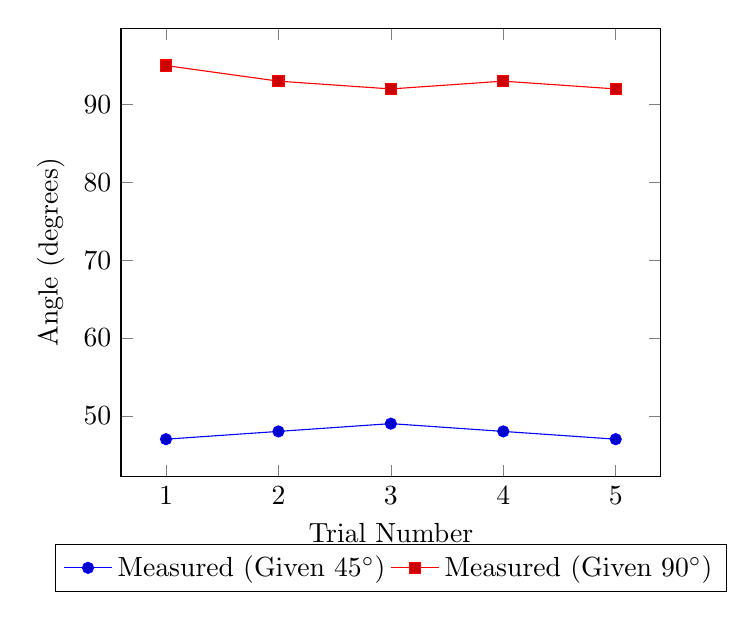
\begin{tikzpicture}
                    \begin{axis}[
                         x tick label style={ /pgf/number format/1000 sep=},
                         ylabel=Angle (degrees),
                         xlabel=Trial Number,
                         legend style={at={(0.5,-0.15)}, anchor=north,legend columns=-1}]
                         \addplot coordinates {(1,47) (2,48) (3,49) (4,48) (5,47)};
                         \addplot coordinates {(1,95) (2,93) (3,92) (4,93) (5,92)};
                         \legend{Measured (Given \SI{45}{\degree}), Measured (Given \SI{90}{\degree})}
                    \end{axis}
               \end{tikzpicture}
               \caption[Measurements of Angle Discrepancy]{Plot of discrepancy between given angle and measured angle.}
               \label{fig:measured-plot}
          \end{figure}


% Conclusion
     \section{Conclusion}
     \lipsum[1]
     \newpage
% References
     \printbibliography
     \newpage
% Appendix
     \begin{appendices}
          \section{Example}
          \lipsum[1]
          \section{Example}
          \lipsum[1]
     \end{appendices}



\end{document}
